% !TEX root = ../paper.tex
\section{Design}
\subsection{Design Summary}\label{sec:design-summary}
Lean 4 is a good target for our translation as well as a suitable language to implement our translation in because Lean 4 is mostly implemented in itself. As users, we can utilize and emit the same data structures used in Lean's implementation to extend the functionality of Lean \cite{moura2021lean}. These metaprogramming capabilities of Lean make our work implementing a Forge module in Lean much easier. 

The Lean 4 compilation process is structured as in \cref{fig:lean-compilation}. 
\begin{figure}[h!]
\centering
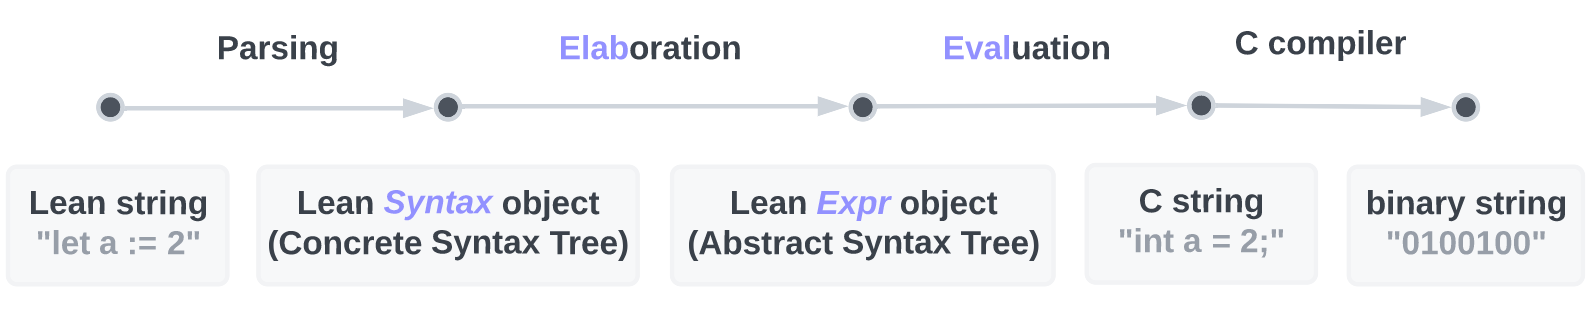
\includegraphics[width=0.8\textwidth]{images/lean-compiler.png}
\caption{A diagram from \cite{metaprogramming} summarizing the Lean 4 compilation process.}
\label{fig:lean-compilation}
\end{figure}

Specifically, the parsing and elaboration steps are designed to be highly customizable and are provided as a `first-class' feature of Lean 4. We approach the problem of translating Forge into Lean as a task of adding new language features to Lean itself. We define our own Lean syntax objects that correspond to a concrete syntax tree (CST) of Forge and implement a parser for Forge (see \cref{sec:parsing}), and then implement a custom elaboration function for our Forge syntax to translate it into native Lean expressions (see \cref{sec:elaboration}). \textsc{Lforge}'s translation process, which is tightly integrated into the Lean compilation process, is outlined in \cref{fig:lforge-process}. 

\begin{figure}[h!]
\centering
% !TEX root = ../../paper.tex

% Source: https://tex.stackexchange.com/questions/376397/create-a-flowchart-style-figure

\begin{tikzpicture}[
    node distance = 3mm and 12mm,
      start chain = going right,
      NTRC/.style = {% Node with Two Rounded Corners
        inner sep=1mm, text width=25mm, minimum height=11mm,
        align=center,
        font=\footnotesize\sffamily\bfseries\linespread{.7}, on chain,
        join=by LA,
        path picture={%
        \draw[semithick, rounded corners=3pt];
                    }%end of path picture
                    },
        L/.style = {% for Labels
        font=\scriptsize\sffamily, align=center
                    },
        LA/.style = {% Line with Arrowhead for join macro
        draw=lightgray, semithick, -Stealth
                    },
        LB/.style = {% Line with Bar head
            draw=lightgray,
            {Bar[width=2mm]}-{Bar[width=2mm]},
            shorten >=-0.5\pgflinewidth, shorten <=-0.5\pgflinewidth,
                    },
    every label/.append style = {L},]
    \node (n1) [NTRC,label={\texttt{\tiny TSyntax `f_program}},fill=forgelistingcolor,rounded corners=3pt] {Forge Syntax};
    \node (n2) [NTRC,label={\texttt{\tiny ForgeModel}},fill=leanimpllistingcolor,rounded corners=3pt] {Forge AST};
    \node (n3) [NTRC,label={\texttt{\tiny Expr}},fill=leanimpllistingcolor,rounded corners=3pt] {Lean AST};
    \node (n4) [NTRC,label={Lean Environment},fill=leanlistingcolor,rounded corners=3pt] {Lean\\[-3pt] Kernel / LSP} ;
    \path (n1) to [L,"Parsing"] (n2);
    \path (n2) to [L,"Elab"] (n3);
    \path (n3) to [L,"Eval"] (n4);
    % \draw[LA] (n4) to [L,"Decoded\\ Output"] node (m4);
    \end{tikzpicture}
    
\caption{A diagram of \textsc{Lforge}'s translation process.}
\label{fig:lforge-process}
\end{figure}  

As a result, there is as little additional overhead as possible when translating a Forge specification in Lean. After users have imported our module, all Forge expressions \emph{are} valid Lean expressions and the two languages can be used interchangeably\footnote{We are very fortunate that there are few to no conflicts between Forge and Lean syntax that would hinder this. We provide a flag \texttt{\#lang forge} following Forge's Racket \texttt{\#lang} syntax when users want to explicitly denote Forge code, and the Lean parser will try to parse as many succeeding lines as Forge as possible.}. Definitions can be passed to and from (see Mixed Execution, \cref{sec:dsl}), and most notably Forge predicates can be proven in Lean. 

\subsection{Syntax, Parsing, and the Forge AST}\label{sec:parsing}
In the case of parsing, by defining the Forge grammar in the same specification format that Lean defines its syntax in, we can rely on Lean's parser to parse Forge source code for us.

The benefits of this are two-sided:
\begin{enumerate}
  \item We are provided \texttt{Syntax}-typed Lean objects at the end of this process, the same type that parsing a Lean program would produce. This enables us to treat our Forge implementation as implementation of additional Lean language features, and we can also harness Lean metaprogramming libraries along the way. This is to say, we are implementing Forge in Lean the \emph{same way} Lean is implemented in Lean, which greatly reduces our burden for additional implementation overhead.
  \item By defining Forge `blocks' as a Lean \texttt{command}---which is the top-level syntax category\footnote{For example, the top-level definition in Lean ``\texttt{def x: Int := 0}'' is a `command'.}---users of the tool can insert raw Forge, without any annotations that this is an ``extension language'', into Lean. With the addition of an import statement, every Forge program \emph{is} a valid Lean program.
\end{enumerate}

Lean allows us to create \emph{syntax categories} for each nonterminal symbol in our grammar. At the top-level, we have defined \texttt{f\_sig} (Sigs), \texttt{f\_pred} (Predicates), \texttt{f\_fun} (Functions). Terms are either \texttt{f\_fmla} for formulas (evaluate to True or False) or \texttt{f\_expr} for expressions (evaluate to a set, relation, int).

For example, the grammar\footnote{Where $,+$ and $,*$ denote one/zero or more comma-separated occurrences respectively. $+$ and $*$ denote one/zero or more repetitions.} of Forge arguments and predicates is:

\vspace{1em}\begin{center}
\begin{minipage}{0.8\textwidth}
\setlength{\grammarindent}{6em}
\begin{grammar}
<arg> ::= <ident>,+ `:' <expr>

<args> ::= <arg>,*

<pred> ::= `pred' <ident> [`[' <args> `]'] `{' <fmla>* `}'
\end{grammar}
\end{minipage}
\end{center}

Which we can translate into a corresponding syntax definition in Lean:
\begin{leanimpl*}
declare_syntax_cat f_arg
syntax ident,+ ":" f_expr : f_arg

declare_syntax_cat f_args
syntax f_arg,* : f_args

declare_syntax_cat f_pred
syntax "pred" ident ("[" f_args "]")? "{" f_fmla* "}" : f_pred
\end{leanimpl*}

Following this blueprint, we can translate the entirety of the grammar of Forge\footnote{At least, a useful subset of the Forge language we care about. This is based off the grammar of Alloy \cite{jackson2012software,jackson2019alloy,ngpdbccdlrrvwwk-oopsla-2024}.} into Lean syntax definitions. This is provided in our package as the \texttt{Lforge.Ast} module (see \cref{appendix:code}).

What remains to be done is to convert syntax, almost one-to-one, into an AST for Forge, and then \emph{elaborate} (see \cref{sec:elaboration}) our AST into Lean expressions and declarations.

\begin{leanimpl*}
structure Predicate where
  name : Symbol
  name_tok : Syntax
  args : List (Symbol × Expression) -- (name, type) pairs
  body : Formula -- with args bound
  deriving Repr, Inhabited   
\end{leanimpl*}

The associated structure definitions of the Forge AST is a deep embedding of Forge into Lean. Our overall parser has type \texttt{TSyntax `f_program → MetaM ForgeModel}\footnote{`Sub-parsers', like the one that parses single predicate declarations, are typed \texttt{TSyntax `f_pred → MetaM Predicate}.}, where \texttt{f_program} is the top-level syntax category for Forge programs (lists of sigs, predicates, and functions), and \texttt{MetaM} is a metaprogramming monad that provides us with error reporting. Using this, we can then implement a translation of our Forge model into native Lean expressions and types. 

\subsection{Elaboration}\label{sec:elaboration}

Elaboration in Lean 4 processes Lean \texttt{Syntax} objects, which are the outputs of the Lean parser, into Lean \texttt{Expr} objects\footnote{Technically, \texttt{Expr} objects wrapped in relevant monads that allow us to implement side-effects, like error and info reporting within the Lean LSP (see \cref{sec:dsl}) and interact with Lean's environment.}, which are Lean's low-level kernel representations \cite{metaprogramming}. Elaboration is responsible for Lean's type and metavariable unification\footnote{That is, types are inferred, coerced, and type classes resolved at this step. Types, including implicit types, and must be fully specified within \texttt{Expr} objects.}, which provides all the type information to Lean. 

The process via which to add new syntax and functionality into Lean is first to define said syntax and then to define custom elaboration functions that take Forge \texttt{Syntax} objects, pass those through the parser to produce a Forge AST object (specifically, typed \texttt{ForgeModel}; see above \cref{sec:parsing}), then ingest the Forge AST and return a \texttt{CommandElabM Unit} type, where the \texttt{CommandElabM} monad allows us to add declarations to the environment (and \texttt{Unit} because we don't expect top-level declarations/commands to return values). 

Our elaboration function takes care of elaborating sigs and fields into their corresponding opaque types (see \cref{sec:sigs}), and creates relevant definitions for predicates and functions, inserts the corresponding translations of formulas and expressions respectively (see below \cref{sec:forge-model}), and adds said definitions into the working Lean environment.

\newpage
\section{The Forge Model in Lean: An Overview}\label{sec:forge-model}
We need to take careful choice of how we use elaboration (see above \cref{sec:elaboration}) to translate Forge concepts into corresponding Lean equivalents. While many of our translations are self-evident, others have complex subtleties. Having the \emph{means} to perform such a translation does not make the task of translation itself any easier. We need to ensure that the translation is coherent and interoperable\footnote{Informally, our translation should be like a homomorphism, preserving the structure of Forge models.}. 

Here we outline the Forge syntax and give an overview of their equivalents in Lean. When there are nuances or specific edge cases in a particular translation, we refer to the appropriate section that addresses them. Where translations have not been implemented, we provide a justification behind this conscious decision. 

This should serve as a birds-eye-view of the entire project, and point to specific instances of translations and implementations mentioned throughout this paper. 

\begin{description}
  \item[Sigs] See \cref{sec:sigs} for a discussion on Forge sigs, how they're translated, and how quantifiers (like \texttt{one} or \texttt{abstract}) are handled.
  \item[Formulas] Formulas evaluate to some \texttt{True} or \texttt{False} value; see \cref{tab:fmlas} for translations of various Forge formulas.
  \item[Expressions] Expressions evaluate to some set-typed expression; see \cref{tab:exprs} for translations of the various Forge expressions. While we treat integers as expressions, they are detailed separately. 
  \item[Predicates and functions] Predicates and functions get mapped to top-level definitions in Lean, with the body being the translated formula or expression respectively. See code listings included in \cref{sec:sigs} for an example with functions and \cref{sec:everything-is-a-set} for an example with predicates. 
  \item[Operations with integers] See \cref{tab:ints} for translations of integer expressions, and additionally \cref{sec:integers} on how integers are specifically handled and implemented. 
\end{description}

% !TEX root = ../../paper.tex

\newpage
\begin{table}[h!]
  \renewcommand{\arraystretch}{1.1}
  \centering
  \caption{A list of Forge formula syntax and their corresponding Lean implementations in \textsc{Lforge}. \texttt{x}, \texttt{y}, and \texttt{z} represent formulas; \texttt{a} and \texttt{b} represent expressions; \texttt{T} represents the sig of expression \texttt{a}; and \texttt{x}, \texttt{y} represent integers.\\}
  \label{tab:fmlas}
  \begin{tabular}{>{\columncolor{forgelistingcolor}}l >{\columncolor{leanlistingcolor}}l@{}}
  \hline
  \cellcolor{white} \textbf{Forge Syntax} &
    \cellcolor{white} \textbf{Lean Implementation} \\ \hline
  \texttt{!x} &
    $\neg \texttt{x}$ \\
  \texttt{x \&\& y} &
    $\texttt{x} \land \texttt{y}$ \\
  \texttt{x || y} &
    $\texttt{x} \lor \texttt{y}$ \\
  \texttt{x => y} &
    $\texttt{x} \to \texttt{y}$ \\
  \texttt{x => y else z} &
    $\texttt{x} \to \texttt{y} \land \neg \texttt{x} \to \texttt{z}$ \\
  \texttt{x <=> y} &
    $\texttt{x} \leftrightarrow \texttt{y}$ \\
  \texttt{some a} &
    $\exists\ \texttt{x : T}, \texttt{a x}$ \\
  \texttt{no a} &
    $\texttt{a} = \emptyset$ \\
  \texttt{one a} &
    $\exists!\ \texttt{x : T}, a = \{x\}$ \\
  \texttt{lone a} &
    $\texttt{one a} \lor \texttt{no a}$ \\
  \texttt{a in b} &
    \emph{Usually $\texttt{a} \in \texttt{b}$ or $\texttt{a} \subseteq \texttt{b}$, but varies, see \cref{sec:join-cross-subset}.} \\
  \begin{tabular}[c]{@{}l@{}}\texttt{x = y}\\ \texttt{a = b}\end{tabular} &
    \begin{tabular}[c]{@{}l@{}}$\texttt{x} = \texttt{y}$\\ \emph{Usually $\texttt{a} = \texttt{b}$, but varies, see \cref{sec:join-cross-subset}.}\end{tabular} \\
  \begin{tabular}[c]{@{}l@{}}\texttt{n < m}\\ \texttt{n <= m}\\ \texttt{n > m}\\ \texttt{n >= m}\end{tabular} &
    \begin{tabular}[c]{@{}l@{}}$\texttt{n} < \texttt{m}$\\ $\texttt{n} \leq \texttt{m}$\\ $\texttt{n} > \texttt{m}$\\ $\texttt{n} \geq \texttt{m}$\end{tabular} \\
  $\texttt{all a : T | \{} \langle \textit{fmla}\rangle \texttt{\}}$ &
    $\forall\ \texttt{a : T}, \langle \textit{fmla}\rangle$ \\
  $\texttt{some a : T | \{} \langle \textit{fmla}\rangle \texttt{\}}$ &
    $\exists\ \texttt{a : T}, \langle \textit{fmla}\rangle$ \\
  \begin{tabular}[c]{@{}l@{}}$\texttt{one a : T | \{} \langle \textit{fmla}\rangle \texttt{\}}$\\ $\texttt{no a : T | \{} \langle \textit{fmla}\rangle \texttt{\}}$\\ $\texttt{lone a : T | \{} \langle \textit{fmla}\rangle \texttt{\}}$\end{tabular} &
    \begin{tabular}[c]{@{}l@{}}\emph{Unimplemented}\footnotemark\\ \emph{Unimplemented}\\ \emph{Unimplemented}\end{tabular} \\
  $\texttt{let a = }\langle\textit{term}\rangle\ \texttt{| ... }$ & $\texttt{let a}:= \langle\textit{term}\rangle \texttt{ in ...}$ \\
  $\langle \textit{pred}\rangle\texttt{[a,...]}$ &
  $\langle \textit{pred}\rangle\ \texttt{a ...}$ \\
  \begin{tabular}[c]{@{}l@{}}\texttt{true}\\ \texttt{false}\end{tabular} &
    \begin{tabular}[c]{@{}l@{}}\texttt{True}\\ \texttt{False}\end{tabular} \\ \hline
  \end{tabular}
  \end{table}
  \footnotetext{Due to the semantics of the `complex quantifiers': their interactions with multiple binders and that they encode extra constraints invisibly \cite{forge-docs}, there is no suitable Lean equivalent. Users are suggested to rewrite their quantification statements using only \texttt{all} and \texttt{some}, which all complex quantifiers can be expressed using.}  
  
\newpage

\begin{table}[h!]
  \renewcommand{\arraystretch}{1.1}
  \centering
  \caption{A list of Forge expression syntax and their corresponding Lean implementations. \texttt{x} represents a formula; and \texttt{a} and \texttt{b} represent expressions.\\[-0.5em]}
  \label{tab:exprs}
  \begin{tabular}{>{\columncolor{forgelistingcolor}}l >{\columncolor{leanlistingcolor}}l@{}}
      \hline
  \cellcolor{white}\textbf{Forge Syntax} & \cellcolor{white}\textbf{Lean Implementation}                     \\ \hline
  \texttt{\~{}a}          & \texttt{Relation.Transpose a} or \texttt{a.swap}\footnotemark \\
  \texttt{\^{}a}          & \texttt{Relation.TransGen a}                     \\
  \texttt{*a}          & \texttt{Relation.ReflTransGen a}                 \\
  \texttt{a + b}        & $\texttt{a} \cup \texttt{b}$                     \\
  \texttt{a - b}        & $\texttt{a} \setminus \texttt{b}$                \\
  \texttt{a \& b}        & $\texttt{a} \cap \texttt{b}$                     \\
  \texttt{a.b} \emph{or} \texttt{b[a]}                           & \emph{Varies, see \cref{sec:join-cross-subset}.}           \\
  \texttt{a->b}         & \emph{Varies, see \cref{sec:join-cross-subset}.}  \\
  \texttt{if x then a else b}                                    & \texttt{if x then a else b} \emph{(or, \texttt{ite x a b})}          \\
  $\texttt{\{ x : T | } \langle\textit{fmla}\rangle \texttt{\}}$ & $\lambda\ \texttt{x} \mapsto \langle\textit{fmla}\rangle$ \\
  $\texttt{let a = }\langle\textit{term}\rangle\ \texttt{| ... }$ & $\texttt{let a}:= \langle\textit{term}\rangle \texttt{ in ...}$ \\
  $\langle \textit{fun} \rangle\texttt{[a,...]}$                 & $\langle \textit{fun} \rangle\ \texttt{a ...}$            \\
  \texttt{\# a}         & \texttt{Set.ncard a}                            \\ \hline
  \end{tabular}
\end{table}
\footnotetext{This depends on the type of \texttt{a}. In the specific case when \texttt{a} is a cross product, we can use \texttt{Prod.swap}.}

\vspace{-1em}
\begin{table}[h!]
  \renewcommand{\arraystretch}{1.1}
  \centering
  \caption{A list of Forge integer-related syntax and their corresponding Lean implementations. \texttt{n, m} represent integers; \texttt{a} represents expressions; and \texttt{T} represents the sig of expression \texttt{a}.\\[-0.5em]}
  \label{tab:ints}
  \begin{tabular}{>{\columncolor{forgelistingcolor}}l >{\columncolor{leanlistingcolor}}l@{}}
      \hline
  \cellcolor{white}\textbf{Forge Syntax} & \cellcolor{white}\textbf{Lean Implementation}                     \\ \hline
  \texttt{sing[a]} & \texttt{(a : ℤ)} \\
  \texttt{sum[a]} & \texttt{Finset.sum a id} \\
  \texttt{max[a]} & \texttt{Finset.max a}\footnotemark \\
  \texttt{min[a]} & \texttt{Finset.min a} \\
  \texttt{abs[n]} & \texttt{Int.natAbs n} \\
  \texttt{sign[n]} & \texttt{Int.sign n} \\
  \texttt{add[n, m, ...]} & \texttt{n + m + ...} \\
  \texttt{subtract[n, m, ...]} & \texttt{n - m - ...} \\
  \texttt{multiply[n, m, ...]} & \texttt{n * m * ...} \\
  \texttt{divide[n, m, ...]} & \texttt{(n / m) / ...} \\
  \texttt{remainder[n, m]} & \texttt{Int.mod n m} \\
  $\texttt{sum a : T | \{} \langle \textit{int-expr} \rangle \texttt{\}}$ & $\texttt{Finset.sum (T : Set T)}\ \langle \textit{int-expr} \rangle$ \\
  \hline
  \end{tabular}
\end{table}
\footnotetext{With slight modifications since behavior can be undefined (can produce $\bot$ or $\top$).}

